% Copyright (c) 2026 Geovana Neves. Licensed under CC BY 4.0 (https://creativecommons.org/licenses/by/4.0/). See LICENSE-AND-AUTHORSHIP.md.
%
% 01-workspaces/text/07-workflows.tex
%
% The workflows part: which run type a row takes, what each costs, and the
% quasi-steady rotor in depth. Read from cases/workflows.py (the registered
% keys), cases/qsteady.py (clocking, validity), docs/workspace-and-workflows.md
% ("The quasi-steady rotor"), reports/RPT-089 (the measurements) and the
% owner's decisions of 0.30.0 for --inflow-fft. The figures are drawn by
% figures/qsteady_reduced_frequency.py on the package's generic test blade.
%
% The count nP is the BLADE's: how many times one blade meets the same
% perturbation in one revolution. Never the blade-passing N P of a fixed
% surface, never the rotor-total balance where only multiples of N P survive.

\section{Choosing a workflow}

\begin{frame}{Four workflows, five ways to solve a row}
\relax % a body opening with a brace group would be read as the frame subtitle
{\ftstablesize\renewcommand{\arraystretch}{1.12}
\begin{tabularx}{\linewidth}{@{}P{0.17\linewidth}P{0.25\linewidth}RP{0.14\linewidth}@{}}
\toprule
\textbf{\code{WORKFLOW}} & \textbf{What is solved} & \textbf{When to use it} & \textbf{Cost} \\
\midrule
\code{steady} & one converged steady solve per point; a sweep is one job &
  a body in a steady flow: polars, sweeps, a fixed wing (FSI with its own
  weight) & seconds per point \\
\code{unsteady} & a march in physical time, nothing turning &
  a flow that changes in time without a rotor: a manoeuvre rate, a start-up,
  a fixed wing coupled per step & minutes \\
\code{unsteady\_rotor} & the blades turn, the wake is shed in time &
  the reference for any rotor: installed, interacting, several rotors, a
  time history, the in-plane loads & minutes to hours \\
\code{qsteady\_rotor}, sector & one blade held still, periodic copies, the
  free stream turning & an isolated, axisymmetric rotor in an inflow the same
  at every azimuth; blade FSI with centrifugal loads & seconds \\
\code{qsteady\_rotor}, wheel & every blade held still; one steady solve per
  clocking, averaged & the same rotor at an angle or in a custom inflow, when
  thrust and torque are what matter & seconds per clocking \\
\bottomrule
\end{tabularx}}
\par\vspace{1mm}
{\scriptsize Every row names its workflow in the \code{WORKFLOW} column; a key
another workflow registers is refused by name at \pyfs{plan}. Costs are orders
of magnitude on one workstation, measured on a six-blade research propeller
[14].\par}
\end{frame}

\begin{frame}{A decision chart}
\centering
\begin{adjustbox}{max width=\linewidth, max totalheight=0.76\textheight}
\begin{tikzpicture}[
  q/.style={draw=CourseBlue, fill=CourseBlue!6, rounded corners=1.5mm,
    align=center, font=\scriptsize, inner sep=1.3mm, text width=5.2cm},
  a/.style={draw=CourseGold, fill=CourseGold!15, align=center,
    font=\scriptsize\ttfamily, inner sep=1.2mm, minimum width=3.3cm},
  e/.style={-{Stealth[length=1.8mm]}, thick, CourseBlue},
  l/.style={font=\tiny, text=SoftGray, fill=white, inner sep=0.5mm},
  n/.style={font=\tiny, text=SoftGray, align=left}]
\node[q] (q1) at (0,0) {Does a rotor turn in the row?};
\node[q] (q2) at (0,-1.45) {An isolated, axisymmetric rotor, and nothing
  else in the flow?};
\node[q] (q3) at (0,-2.9) {Does the inflow vary around the disc (an angle of
  attack or sideslip, an azimuthal custom field)?};
\node[q] (q4) at (0,-4.35) {Are thrust and torque the answer, and \(k\) small
  over most of the span?};
\node[a] (a1) at (6.0,0) {steady {\normalfont or} unsteady};
\node[n, right=1.5mm of a1] {unsteady when the flow\\changes in time};
\node[a] (a2) at (6.0,-1.45) {unsteady\_rotor};
\node[n, right=1.5mm of a2] {an airframe, several\\rotors, a wing nearby};
\node[a] (a3) at (6.0,-2.9) {qsteady\_rotor, sector};
\node[n, right=1.5mm of a3] {an inflow varying with the\\radius alone; FSI allowed};
\node[a] (a4) at (6.0,-4.35) {qsteady\_rotor, wheel};
\node[n, right=1.5mm of a4] {\code{PASSAGE\_POSITIONS: k},\\mandatory};
\node[a] (a5) at (0,-5.65) {unsteady\_rotor};
\node[n, right=1.5mm of a5] {in-plane loads, a history, a large \(k\)};
\draw[e] (q1) -- node[l] {no} (a1);
\draw[e] (q1) -- node[l] {yes} (q2);
\draw[e] (q2) -- node[l] {no} (a2);
\draw[e] (q2) -- node[l] {yes} (q3);
\draw[e] (q3) -- node[l] {no} (a3);
\draw[e] (q3) -- node[l] {yes} (q4);
\draw[e] (q4) -- node[l] {yes} (a4);
\draw[e] (q4) -- node[l] {no} (a5);
\end{tikzpicture}
\end{adjustbox}
\par\vspace{1mm}
{\scriptsize \(k\) is the blade's 1P reduced frequency (Part ``the quasi-steady
rotor''); \pyfs{plan} prints it for every wheel point.\par}
\end{frame}

\begin{frame}{\code{steady} and \code{unsteady}}
\begin{columns}[T]
\begin{column}{0.48\textwidth}
\begin{block}{\code{steady}}
\small One converged solve per point; an \code{ALPHA:sweep} or
\code{BETA:sweep} row is one job, every point starting cold unless
\code{COLD\_START: false}. The polar, the super file and the sections are
instants of the last iteration. A custom inflow (\code{FREESTREAM}) or a
free-stream rate (\code{roll\_rate}, \code{pitch\_rate}, \code{yaw\_rate})
is still one steady solve.
\end{block}
\end{column}
\begin{column}{0.48\textwidth}
\begin{block}{\code{unsteady}}
\small A march of \code{TIME\_ITERATIONS} steps of \code{DELTA\_TIME}, and
the window it is averaged over, \code{LAST\_ITERS\_AVG}, which the row must
state. Nothing turns but the free stream; a rotor is
\code{unsteady\_rotor}'s. The products are averages over the window, and the
history is kept.
\end{block}
\end{column}
\end{columns}
\begin{takeaway}The window belongs to the row, not to the pproc: changing it
is a new \pyfs{post}, never a new run (Guide 5).\end{takeaway}
\end{frame}

\begin{frame}{\code{unsteady\_rotor}: the reference, and its price}
\begin{columns}[T]
\begin{column}{0.52\textwidth}
\begin{itemize}\small
  \item The blades turn at \code{RPM} (or from \code{ADVANCE\_RATIO}), about
        the rotor block's axis, with its hand; the step is \code{DELTA\_THETA}
        degrees or \code{DELTA\_TIME}, the length \code{REVOLUTIONS} or
        \code{TIME\_ITERATIONS}, and \code{LAST\_REVS\_AVG} is mandatory.
  \item The only workflow for a rotor on an airframe, for several rotors
        (\code{MOTIONS}), for the time history and phase-locked products, and
        the one to trust for the in-plane loads.
  \item FSI is refused on it in this release (Guide 6).
\end{itemize}
\end{column}
\begin{column}{0.44\textwidth}
\begin{alertblock}{A few revolutions are not a developed wake}
\small On a six-blade research propeller the thrust still rose about
0.5\,\% per revolution at revolution 6 [14]. A window over the third of three
revolutions averages a wake still growing: run more revolutions before the
window when the level matters, and compare points at the same revolution
count when the difference matters.
\end{alertblock}
\end{column}
\end{columns}
\end{frame}

\section{The quasi-steady rotor}

\begin{frame}{\code{qsteady\_rotor}: a rotor solved steady}
\begin{columns}[T]
\begin{column}{0.50\textwidth}
\begin{itemize}\small
  \item \textbf{One workflow, for an isolated, axisymmetric rotor only.} The
        blades stay still; the free stream turns about the shaft at the
        rotor's speed (\code{SET\_FREESTREAM ROTATION}, the hub frame, the
        shaft, the signed speed); every solve is steady.
  \item The reference declares exactly one rotor block; the row states
        \code{RPM} or \code{ADVANCE\_RATIO}. A second rotor, an actuator disc,
        a body rate, or a boundary that is none of the rotor's is refused.
  \item \textbf{Sector}: \code{SYMMETRY} periodic, with
        \code{PERIODIC\_COPIES}: the meshed blade once. \textbf{Wheel}: no
        symmetry, every blade meshed. \code{MIRROR} is refused.
\end{itemize}
\end{column}
\begin{column}{0.46\textwidth}
\begin{block}{Why it stands for the turning blade}
\small One blade held still in the rotating free stream against the same
blade turning, after one revolution at the same azimuth: axial force within
0.35\,\%, in-plane force within 2.5\,\% [14].
\end{block}
\begin{takeaway}It is callable without FSI. FSI is its optional right-hand
variable, on the sector only (Guide 6).\end{takeaway}
\end{column}
\end{columns}
\end{frame}

\begin{frame}{Sector or wheel: what the inflow allows}
\begin{columns}[T]
\begin{column}{0.48\textwidth}
\begin{block}{Sector}
\small Stands for the wheel only in an inflow the \textbf{same at every
azimuth}. An angle of attack or of sideslip is refused. A custom inflow
(\code{FREESTREAM}) is accepted only where it varies with the radius alone:
rows at one distance from the shaft state one axial, radial and swirl
velocity. FSI allowed: the structural solver applies the centrifugal loads at
the free-stream rotation's rpm.
\end{block}
\end{column}
\begin{column}{0.48\textwidth}
\begin{block}{Wheel}
\small In an axial, uniform inflow it is steady in the rotating frame: one
solve. At an angle, or in a custom inflow that varies around the disc, each
blade meets another flow: \code{PASSAGE\_POSITIONS: k} is \textbf{mandatory}.
A custom inflow file is the \textbf{total} velocity of the air, in the global
frame; the package writes \(\mathbf{v} - \boldsymbol{\Omega} \times
(\mathbf{p} - \mathbf{p}_\mathrm{hub})\) into a new file and never touches
yours. FSI refused.
\end{block}
\end{column}
\end{columns}
\end{frame}

\begin{frame}{\code{PASSAGE\_POSITIONS}: clockings inside one passage}
\begin{columns}[T]
\begin{column}{0.44\textwidth}
\begin{itemize}\small
  \item \(k\) steady solves, the wheel clocked by
        \[ \theta_i = \frac{i\,(360^\circ/N)}{k}, \quad i = 0 \ldots k-1, \]
        uniform inside ONE blade passage: a wheel of \(N\) alike blades
        repeats every \(360^\circ/N\).
  \item Clocking 0 is solved last with every export; clocking \(i\) leaves
        \code{<point>\_qs<i>.txt}. The post averages them: the products are
        those of an unsteady point.
  \item \textbf{Guidance}: 2 for thrust and torque; 6 or more for the
        in-plane loads.
\end{itemize}
\end{column}
\begin{column}{0.52\textwidth}
{\ftstablesize\renewcommand{\arraystretch}{1.05}
\begin{tabular*}{\linewidth}{@{\extracolsep{\fill}}rrrrr@{}}
\toprule
\(k\) & \(F_x\) [N] & \(F_y\) [N] & \(F_z\) [N] & \(M_z\) [N m] \\
\midrule
1 & \(-2210.56\) & \(-23.37\) & 258.84 & \(-347.98\) \\
2 & \(-2206.12\) & \(-23.81\) & 257.17 & \(-346.05\) \\
3 & \(-2207.84\) & \(-27.53\) & 260.58 & \(-348.87\) \\
6 & \(-2204.64\) & \(-27.09\) & 257.75 & \(-345.45\) \\
12 & \(-2203.95\) & \(-27.46\) & 258.21 & \(-345.95\) \\
24 & \(-2203.82\) & \(-27.57\) & 258.23 & \(-345.95\) \\
\bottomrule
\end{tabular*}}
\par\vspace{1mm}
{\scriptsize A six-blade research propeller at 5\(^\circ\), 26.124 [14]:
\(F_x\) and \(M_x\) within 0.2\,\% from \(k = 2\); at \(k = 6\) every
component within 1.6\,\% of \(k = 24\). About 1.7 s per clocking.\par}
\end{column}
\end{columns}
\end{frame}

\begin{frame}{Is a quasi-steady answer valid? The reduced frequency}
\begin{columns}[T]
\begin{column}{0.52\textwidth}
\begin{itemize}\small
  \item A wheel point at an angle sees its inflow change once per
        revolution. Each blade station's \textbf{1P reduced frequency},
        \[ k = \frac{\Omega\,c}{2\,V_\mathrm{rel}}
             = \frac{\pi c / 2R}{\sqrt{J^2 + \pi^2 (r/R)^2}}, \]
        compares the time the flow takes to cross half a chord with the
        period of that change: below about 0.05 the lag of the circulation
        and the shed wake is small; above 0.1 it is not [10, 11, 12].
  \item It depends on \(J\) and the chord alone, never on the speed: the
        same \(J\) at another Mach number gives the same \(k\).
\end{itemize}
\end{column}
\begin{column}{0.44\textwidth}
\begin{block}{What the package states}
\small \pyfs{plan}: four values per wheel point, the per cent of the span
with \(k > 0.1\) and \(k\) minimum, maximum and mean; a \textbf{warning} when
that per cent is above zero, never a refusal.\\[1mm]
\code{<point>\_qsteady.json}: \(k\) min, max, mean, the span above 0.05 and
0.1, the shares of thrust and torque from stations above 0.1; every product
of the point carries them, the sections product \(k\) per station.
\end{block}
\end{column}
\end{columns}
\end{frame}

\begin{frame}{The reduced frequency of the package's test blade}
\begin{columns}[T]
\begin{column}{0.49\textwidth}
\centering
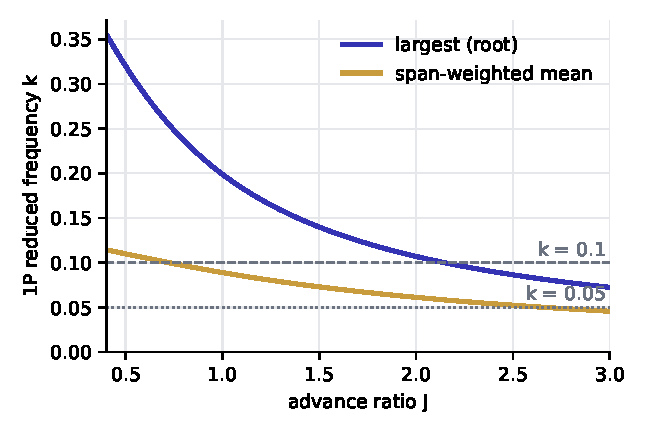
\includegraphics[width=\linewidth]{figures/qsteady_k_vs_J.pdf}
\end{column}
\begin{column}{0.49\textwidth}
\centering
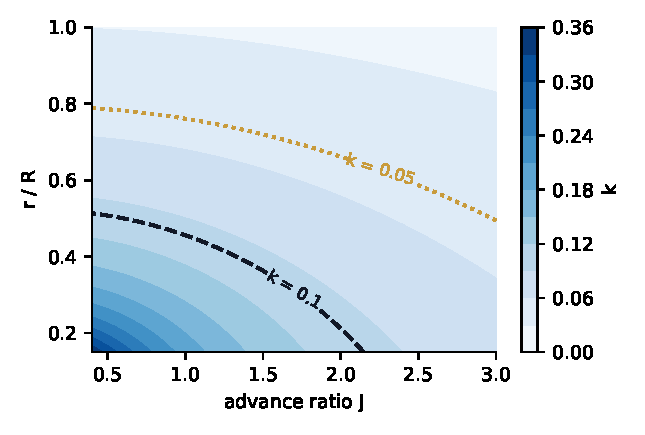
\includegraphics[width=\linewidth]{figures/qsteady_k_map_J_r.pdf}
\end{column}
\end{columns}
\par\vspace{1mm}
{\ftstablesize\renewcommand{\arraystretch}{1.0}
\begin{tabular*}{\linewidth}{@{\extracolsep{\fill}}lrrrrrr@{}}
\toprule
\(J\) & 0.6 & 1.0 & 1.4 & 1.7 & 2.2 & 3.0 \\
\midrule
\(k\) largest (root) & 0.288 & 0.199 & 0.149 & 0.125 & 0.098 & 0.072 \\
span with \(k > 0.1\) [\%] & 41.5 & 36.4 & 28.0 & 19.5 & 0 & 0 \\
\bottomrule
\end{tabular*}}
\par\vspace{0.5mm}
{\tiny\color{SoftGray} The tier-3 blade of the repository (NACA 4409, \(R\) =
1.8288 m, chord over \(R\) from 0.14 at the hub to 0.06 at the tip), from its
chord law; drawn by \code{figures/qsteady\_reduced\_frequency.py}. The root
is the worst station: short radius, wide chord.\par}
\end{frame}

\begin{frame}{What \(n\)P counts: the blade's own count}
\begin{columns}[T]
\begin{column}{0.50\textwidth}
\begin{itemize}\small
  \item \textbf{\(n\)P is counted by ONE blade}: how many times that blade
        meets the same perturbation in one revolution. An angle of attack
        is 1P; a field with four lobes around the disc is 4P, for every blade
        alike.
  \item It is \textbf{not} what a fixed surface near the rotor feels: a wing
        behind it is struck each time any of the \(N\) blades passes, so it
        counts \(N\)P (blade passing).
  \item It is \textbf{not} what a balance under the whole rotor measures:
        summing \(N\) alike blades cancels every harmonic but the multiples
        of \(N\), so only \(m\,N\)P survive there [12].
\end{itemize}
\end{column}
\begin{column}{0.46\textwidth}
\centering
\begin{tikzpicture}[x=0.95cm, y=0.55cm, font=\tiny]
  \foreach \row/\lab in {0/{one blade: 1P and 3P}, -2.3/{a fixed surface: \(N\)P, \(N = 4\)}, -4.6/{the rotor balance: \(m\,N\)P only}} {
    \draw[SoftGray, ->] (0,\row) -- (4.3,\row) node[right] {\(\psi\)};
    \node[anchor=west, text=SoftGray] at (0,\row+1.05) {\lab};
  }
  \draw[CourseBlue, thick, domain=0:360, samples=90]
    plot ({\x/90}, {0.55*sin(\x) + 0.25*sin(3*\x)});
  \draw[CourseGold, thick, domain=0:360, samples=90]
    plot ({\x/90}, {-2.3 + 0.7*abs(sin(2*\x))^6});
  \draw[CourseBlue!70!black, thick, domain=0:360, samples=90]
    plot ({\x/90}, {-4.6 + 0.12*sin(4*\x)});
  \node[text=SoftGray] at (2,-5.5) {one revolution};
\end{tikzpicture}
\end{column}
\end{columns}
\end{frame}

\begin{frame}{\code{--inflow-fft}: how many clockings a custom inflow needs}
\begin{columns}[T]
\begin{column}{0.54\textwidth}
\begin{itemize}\small
  \item A plan option, for \code{qsteady\_rotor} wheel rows with a custom
        inflow: at each radius, the Fourier series in azimuth of the angle
        of attack the \textbf{blade} meets, harmonic \(n\) being \(n\)P in the
        blade's count.
  \item \(n_{95}\): the harmonics holding 95\,\% of that perturbation;
        \(k_\mathrm{eff} = n_{95}\,k_\mathrm{1P}\), reported as minimum,
        maximum, mean and the span with \(k_\mathrm{eff} > 0.1\). With the
        option the validity warning reads \(k_\mathrm{eff}\).
  \item The suggested
        \( \code{PASSAGE\_POSITIONS} \ge n_\mathrm{max}/N + 1 \),
        and a warning when the row states fewer.
\end{itemize}
\end{column}
\begin{column}{0.42\textwidth}
\begin{block}{Why \(n_\mathrm{max}/N + 1\)}
\small The wheel's total load holds only \(m\,N\)P. \(k\) uniform clockings
inside one passage average away every \(m\,N\)P with \(m\) not a multiple of
\(k\); the first one that survives is \(k\,N\)P. So the average is clean when
\(k\,N > n_\mathrm{max}\): a blade harmonic above that aliases into the
mean.
\end{block}
\end{column}
\end{columns}
\end{frame}

\begin{frame}{What to expect against \code{unsteady\_rotor}}
\relax % a body opening with a brace group would be read as the frame subtitle
{\ftstablesize\renewcommand{\arraystretch}{1.15}
\begin{tabularx}{\linewidth}{@{}P{0.16\linewidth}P{0.34\linewidth}R@{}}
\toprule
\textbf{Component} & \textbf{qsteady against unsteady} & \textbf{Why, and what moves it} \\
\midrule
\(F_x\), \(M_x\) (thrust, torque) & \textbf{larger in magnitude}: 7 to 9\,\%
  at 10\(^\circ\) steps and 3 to 6 revolutions & the steady wake is the developed
  one; the unsteady run is still approaching it, so the gap
  \textbf{shrinks} with finer time steps and more revolutions \\
\(F_z\), \(M_z\) (normal force, yawing moment) & \textbf{smaller in
  magnitude}, by roughly 8 to 20\,\% & the phase and level of the 1P blade
  load on the downgoing half of the disc: the lag a steady solve does not
  have \\
\(F_y\), \(M_y\) (side force, pitching moment) & \textbf{unreliable}: tens of
  N against a clocking noise of about 13 N, and they may flip sign & small
  resultants of large blade loads; more clockings do not close the gap \\
\bottomrule
\end{tabularx}}
\par\vspace{1mm}
{\scriptsize A six-blade research propeller at 5\(^\circ\) on 26.124 [14]. At
0\(^\circ\) the same axial gap appears (\(-7.5\,\%\) against 6 revolutions),
so it is the wake, not the angle. Use \code{qsteady\_rotor} for thrust,
torque and trends; use \code{unsteady\_rotor} for the in-plane loads.\par}
\end{frame}

\begin{frame}{The tests behind it}
\begin{columns}[T]
\begin{column}{0.60\textwidth}
{\ftstablesize\renewcommand{\arraystretch}{1.05}
\begin{tabular*}{\linewidth}{@{\extracolsep{\fill}}lrrr@{}}
\toprule
 & U, last rev & Q, 6 clockings & \((Q-U)/|U|\) \\
\midrule
\(F_x\) [N] & \(-2022.76\) & \(-2204.64\) & \(-8.99\,\%\) \\
\(F_y\) [N] & 55.36 & \(-27.09\) & opposite sign \\
\(F_z\) [N] & 320.52 & 257.75 & \(-19.6\,\%\) \\
\(M_x\) [N m] & \(-2274.67\) & \(-2433.44\) & \(-6.98\,\%\) \\
\(M_y\) [N m] & \(-54.83\) & 44.68 & opposite sign \\
\(M_z\) [N m] & \(-410.73\) & \(-345.45\) & \(+15.9\,\%\) \\
\midrule
\(C_T\), \(C_P\) & 0.2903, 0.5623 & 0.3164, 0.6015 & \(+9.0\), \(+7.0\,\%\) \\
wall time & 102.7 s & 10.8 s & \\
\bottomrule
\end{tabular*}}
\par\vspace{0.5mm}
{\tiny\color{SoftGray} U: all six blades turning, 10\(^\circ\) per step, three
revolutions, the last averaged. Q: blades still, six clockings. RPT-089
[14].\par}
\end{column}
\begin{column}{0.37\textwidth}
\begin{ftsevidence}[The time step closes the axial gap]
\scriptsize Same propeller, a later time-step study (not yet a numbered
report): at 0\(^\circ\) and 3 revolutions the axial gap is 8.4\,\% at
10\(^\circ\) per step, 6.6\,\% at 5\(^\circ\), 4.0\,\% at 2.5\(^\circ\); 3.9\,\%
at 5\(^\circ\) and 6 revolutions. At 5\(^\circ\) incidence, 5\(^\circ\) steps,
6 revolutions: \(F_x\) 3.6\,\%, \(F_z\) 11.7\,\%, \(M_z\) 8.2\,\% apart, the
side force and pitching moment still of opposite sign. No step size levelled
off.
\end{ftsevidence}
\end{column}
\end{columns}
\end{frame}

\begin{frame}{Cost, side by side}
\relax % a body opening with a brace group would be read as the frame subtitle
{\ftstablesize\renewcommand{\arraystretch}{1.15}
\begin{tabularx}{\linewidth}{@{}P{0.28\linewidth}P{0.22\linewidth}R@{}}
\toprule
\textbf{The same rotor point} & \textbf{Wall time, one launch} & \textbf{What it buys} \\
\midrule
\code{qsteady\_rotor} wheel, 6 clockings & 10.8 s & thrust and torque; in-plane
  loads as estimates \\
\code{qsteady\_rotor} wheel, 24 clockings & about 42 s & the same, the
  clocking noise below 0.5\,\% \\
\code{unsteady\_rotor}, 10\(^\circ\), 3 revolutions & 102.7 s & the history,
  every component, a wake still developing \\
\code{unsteady\_rotor}, 5\(^\circ\), 6 revolutions & about 18 min & the axial
  gap to the steady wake down to about 4\,\% \\
\bottomrule
\end{tabularx}}
\par\vspace{1.5mm}
\begin{takeaway}Seconds against minutes: sweep \(J\), the angle and the
geometry with \code{qsteady\_rotor}, then confirm the points that matter,
and every in-plane load, with \code{unsteady\_rotor}.\end{takeaway}
{\scriptsize Six-blade research propeller, 26.124, licence checkout included
[14]; the 18 min is the time-step study of the previous frame.\par}
\end{frame}
